\begin{tikzpicture}[x=1pt,y=1pt,
    every node/.style={font=\footnotesize},
    ah/.style={draw opacity=0,line width=0.08,fill opacity=1},
    ahs/.style={ah,scale=0.55},
    lbl/.style={fill=white,align=center,inner sep=2.5pt,line width=0.6pt},
    dim/.style={fill=white,align=center,inner sep=2pt,draw=none,font=\scriptsize},
    pan/.style={font=\footnotesize\bfseries,inner sep=0pt,anchor=north}]

% =========================================================================
% (a)  bottom shell  --  image x: 59.5 -> 237.25 , y: 172 -> 308.9
% =========================================================================
\node [anchor=south west,inner sep=0] at (59.5,172)
  {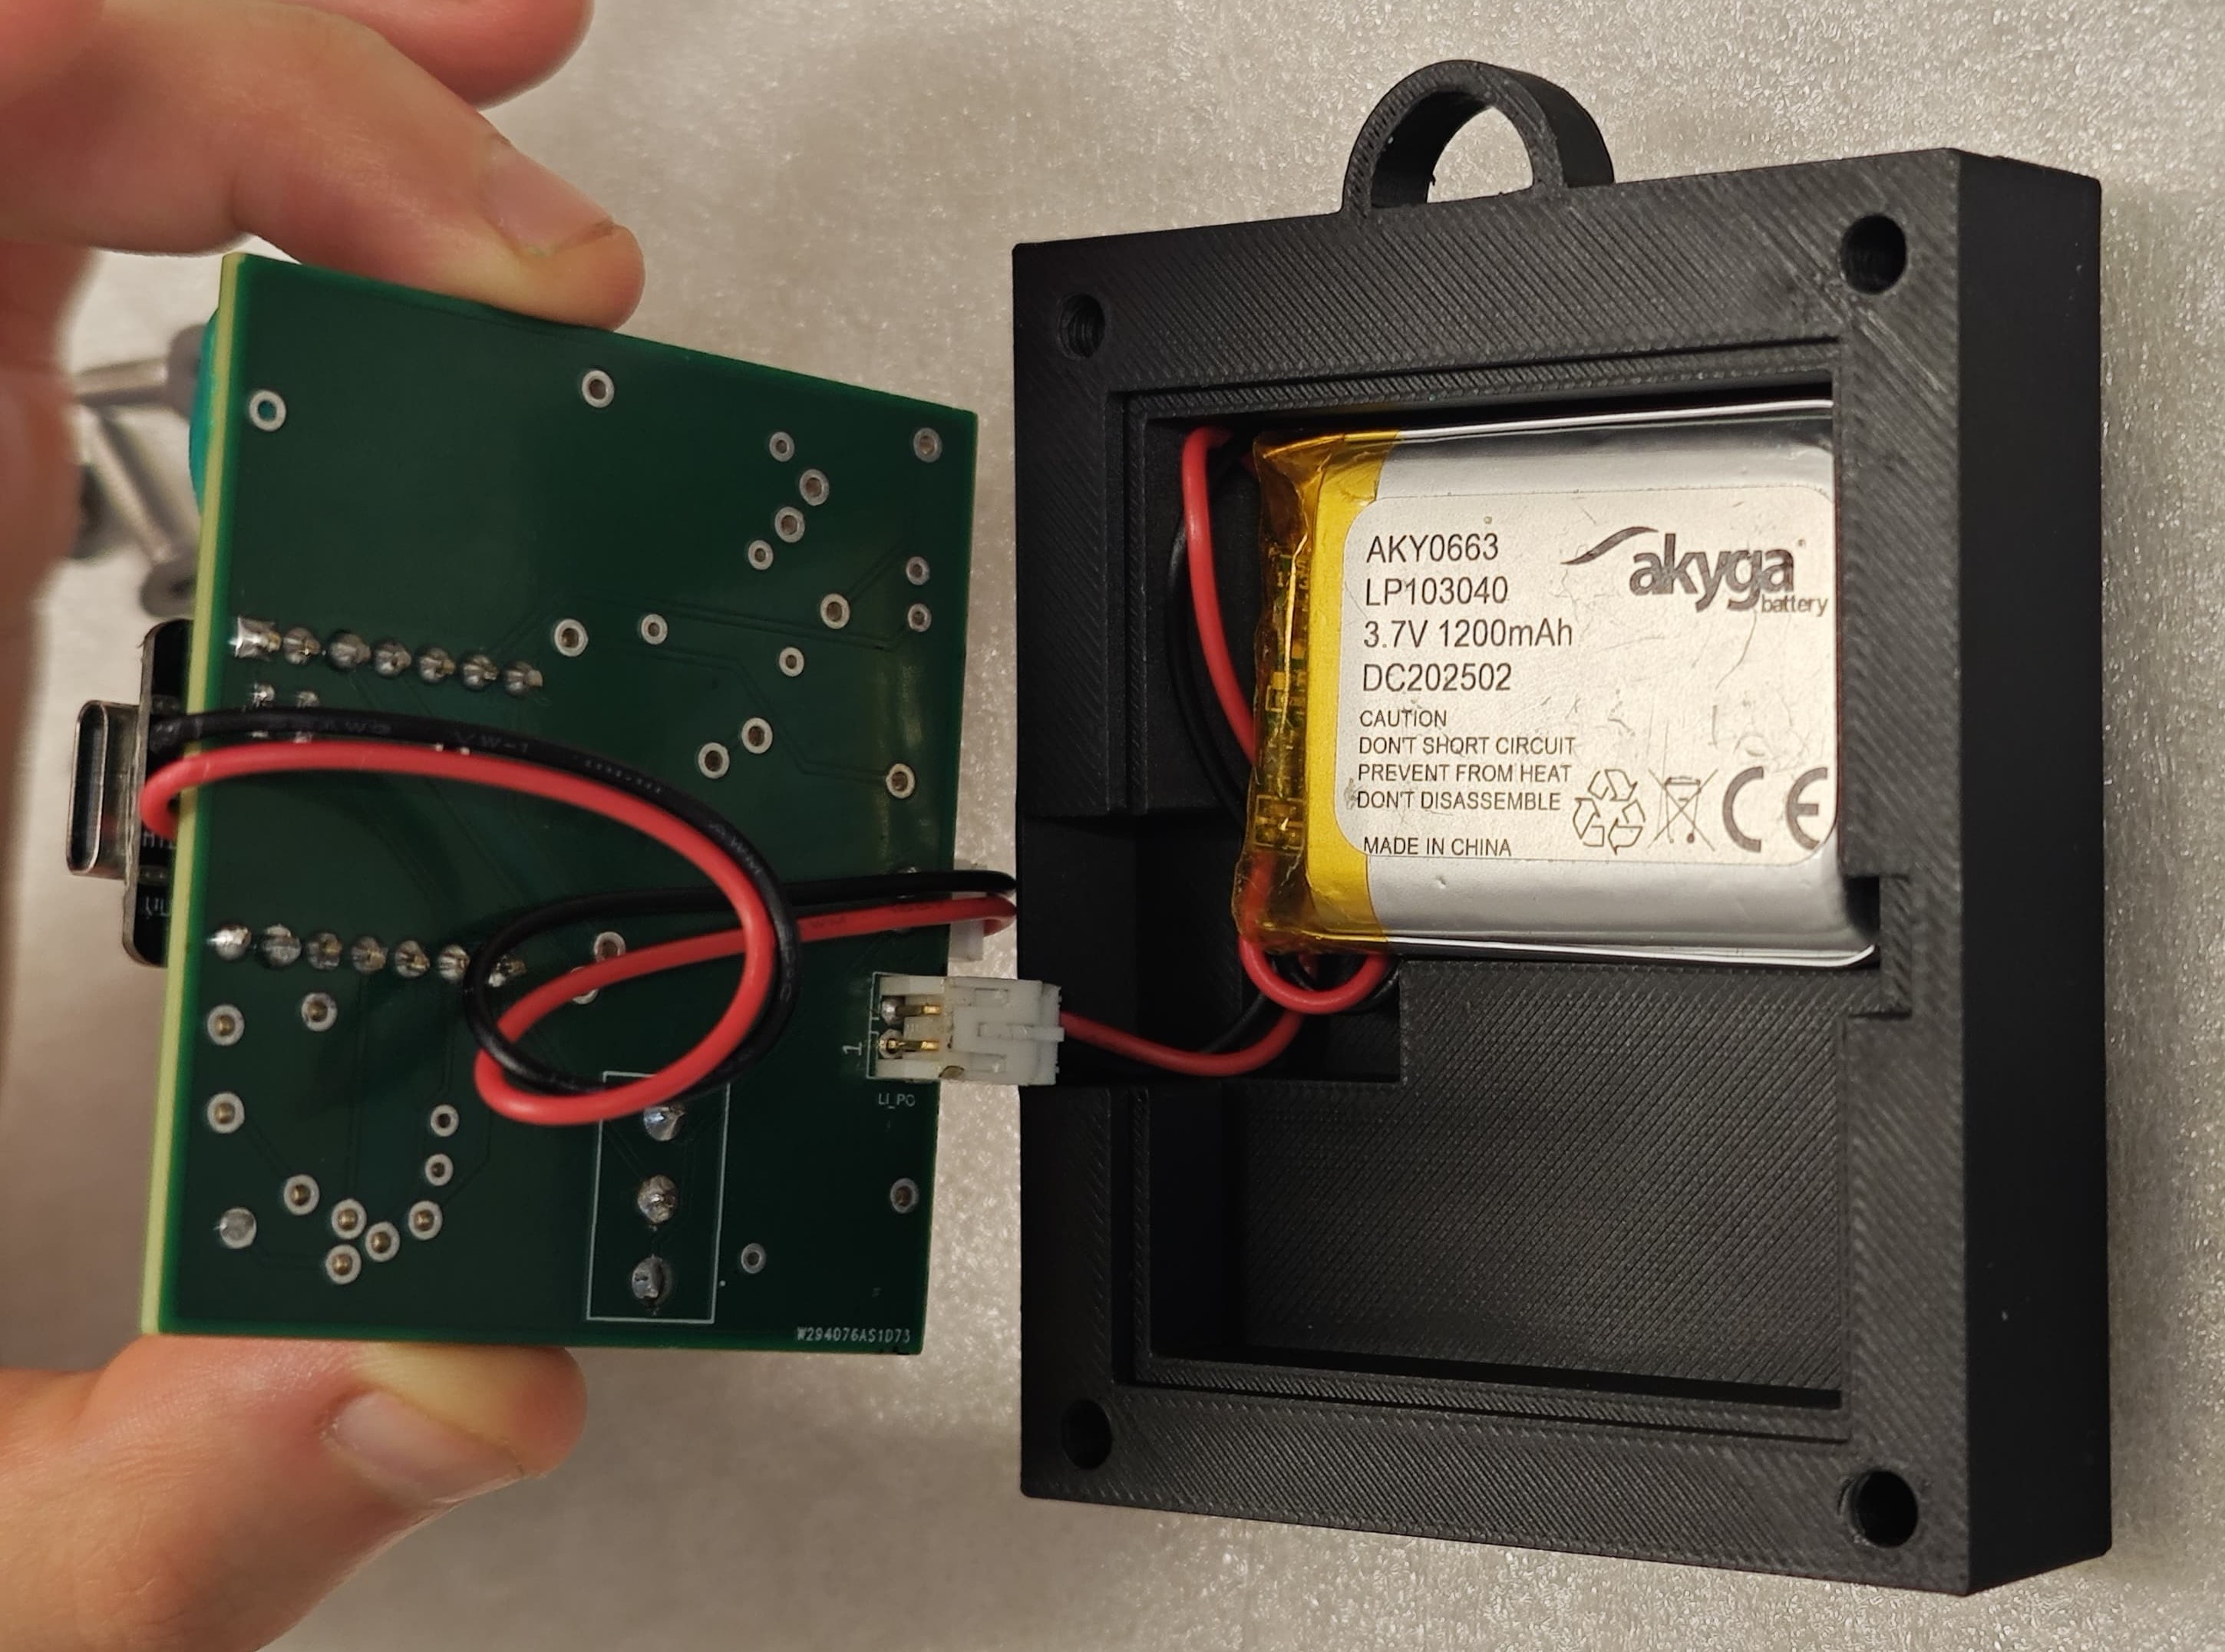
\includegraphics[width=177.75pt,height=136.9pt]{images/baixo.jpg}};

% ---- Battery + cables compartment ---------------------------------------
\node [lbl,draw={rgb, 255:red, 81; green, 81; blue, 81 },anchor=center]
      (batt) at (106.1,280.6) {Battery + Cables\\Compartment};
\draw [color={rgb, 255:red, 81; green, 81; blue, 81 },line width=1.1pt]
      ([xshift=12.5pt]batt.south) -- (147.0,240.4);
\draw [shift={(152.6,234.7)},rotate=134.3,ah,
       fill={rgb, 255:red, 81; green, 81; blue, 81 }]
      (7.85,-3.78) -- (0,0) -- (7.85,3.78) -- cycle ;

% ---- Power cables -------------------------------------------------------
\node [lbl,draw={rgb, 255:red, 241; green, 74; blue, 64 },anchor=center]
      (pcab) at (163.25,189.1) {Power\\Cables};
\draw [color={rgb, 255:red, 241; green, 74; blue, 64 },line width=1.1pt]
      ([xshift=-8pt]pcab.north) -- (151.0,213.7);
\draw [shift={(148.6,221.35)},rotate=287.4,ah,
       fill={rgb, 255:red, 241; green, 74; blue, 64 }]
      (7.85,-3.78) -- (0,0) -- (7.85,3.78) -- cycle ;
\draw [color={rgb, 255:red, 241; green, 74; blue, 64 },line width=1.1pt]
      ([xshift=-8pt]pcab.north) -- (126.4,217.7);
\draw [shift={(119.6,221.85)},rotate=328.6,ah,
       fill={rgb, 255:red, 241; green, 74; blue, 64 }]
      (7.85,-3.78) -- (0,0) -- (7.85,3.78) -- cycle ;

% ---- Panel letter (centred on the image) --------------------------------
\node [pan] at (148.375,164) {(a)};
\begin{scope}[yshift=8pt]
% =========================================================================
% (b)  middle shell  --  image x: 0 -> 135.7 , y: 0 -> 146
% =========================================================================
\node [anchor=south west,inner sep=0] at (0,0)
  {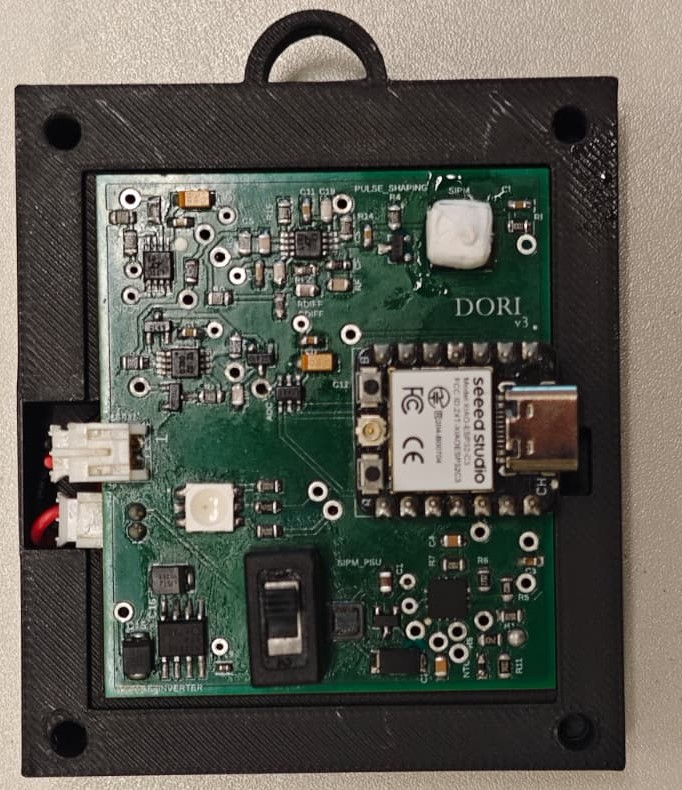
\includegraphics[width=135.7pt,height=146pt]{images/meio.jpg}};

% ---- Teflon-wrapped scintillator ---------------------------------------
\node [lbl,draw={rgb, 255:red, 26; green, 111; blue, 223 },anchor=center]
      (tefl) at (56.65,126.2) {Teflon-wrapped\\Scintillator};
\draw [color={rgb, 255:red, 26; green, 111; blue, 223 },line width=1.1pt]
      ([xshift=9.35pt]tefl.south) -- (79.2,107.0);
\draw [shift={(86.0,102.8)},rotate=148.2,ah,
       fill={rgb, 255:red, 26; green, 111; blue, 223 }]
      (7.85,-3.78) -- (0,0) -- (7.85,3.78) -- cycle ;

% ---- Width dimension (6.3 cm) ------------------------------------------
\draw [line width=1.1pt,black] (2,-4) -- (123.5,-4);
\draw [shift={(2,-4)},rotate=0,ah,fill=black]
      (7.85,-3.78) -- (0,0) -- (7.85,3.78) -- cycle ;
\draw [shift={(123.5,-4)},rotate=180,ah,fill=black]
      (7.85,-3.78) -- (0,0) -- (7.85,3.78) -- cycle ;
\node [dim,anchor=center] at (62.8,-4) {6.3~cm};
% ---- Height dimension (7.2 cm) -----------------------------------------
\draw [line width=1.1pt,black] (-4,3.5) -- (-4,132.5);
\draw [shift={(-4,3.5)},rotate=90,ah,fill=black]
      (7.85,-3.78) -- (0,0) -- (7.85,3.78) -- cycle ;
\draw [shift={(-4,132.5)},rotate=270,ah,fill=black]
      (7.85,-3.78) -- (0,0) -- (7.85,3.78) -- cycle ;
\node [dim,anchor=center,rotate=90] at (-4,68) {7.2~cm};

% ---- Panel letter -------------------------------------------------------
\node [pan] at (67.85,-10) {(b)};

% =========================================================================
% (c)  top shell  --  image x: 159.7 -> 296.8 , y: 0 -> 146
% =========================================================================
\node [anchor=south west,inner sep=0] at (159.7,0)
  {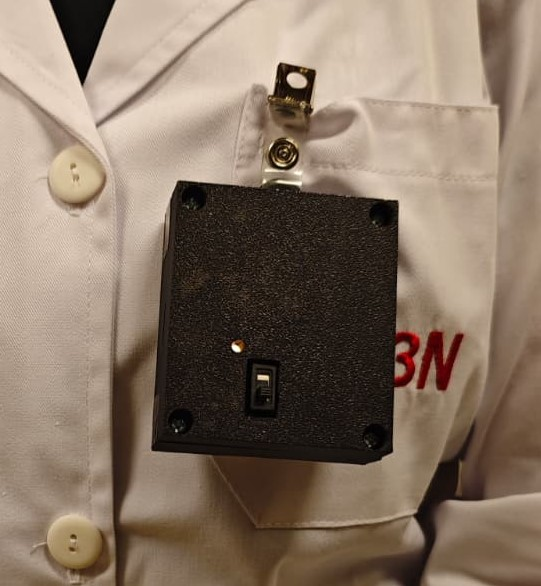
\includegraphics[width=137.1pt,height=146pt]{images/cima.jpg}};
% ---- LED --------------------------------------------------------------
\node [lbl,draw={rgb, 255:red, 204; green, 153; blue, 0 },anchor=center]
      (led) at (181.75,71.45) {LED On};
\draw [color={rgb, 255:red, 204; green, 153; blue, 0 },line width=1.1pt]
      (led.east) -- (217.6,61.6);
\draw [shift={(219.5,60.4)},rotate=151.2,ah,
       fill={rgb, 255:red, 204; green, 153; blue, 0 }]
      (7.85,-3.78) -- (0,0) -- (7.85,3.78) -- cycle ;
% ---- Badge clip ---------------------------------------------------------
\node [lbl,draw={rgb, 255:red, 55; green, 173; blue, 107 },anchor=center]
      (badge) at (269.4,107.7) {Badge Clip};
\draw [color={rgb, 255:red, 55; green, 173; blue, 107 },line width=1.1pt]
      (badge.north) -- (245.3,120.7);
\draw [shift={(237.5,122.6)},rotate=346.6,ah,
       fill={rgb, 255:red, 55; green, 173; blue, 107 }]
      (7.85,-3.78) -- (0,0) -- (7.85,3.78) -- cycle ;


% ---- Power switch -------------------------------------------------------
\node [lbl,draw={rgb, 255:red, 241; green, 74; blue, 64 },anchor=center]
      (psw) at (265.15,47) {Power\\Switch};
\draw [color={rgb, 255:red, 241; green, 74; blue, 64 },line width=1.1pt]
      (psw.west) -- (240,47);
\draw [shift={(232,47)},rotate=0,ah,
       fill={rgb, 255:red, 241; green, 74; blue, 64 }]
      (7.85,-3.78) -- (0,0) -- (7.85,3.78) -- cycle ;

% ---- Thickness dimension (2.5 cm, short arrow -> scaled heads) ----------
\draw [line width=1.1pt,black] (201.0,92.9) -- (205.8,101.6);
\draw [shift={(201.0,92.9)},rotate=61.1,ahs,fill=black]
      (7.85,-3.78) -- (0,0) -- (7.85,3.78) -- cycle ;
\draw [shift={(205.8,101.6)},rotate=241.1,ahs,fill=black]
      (7.85,-3.78) -- (0,0) -- (7.85,3.78) -- cycle ;
\node [dim,anchor=center,rotate=61] at (194.7,102.2) {2.5~cm};
% ---- Panel letter -------------------------------------------------------
\node [pan] at (228.25,-10) {(c)};
\end{scope}
\end{tikzpicture}